\documentclass[11pt]{article}
\usepackage[margin=1in]{geometry}
\usepackage[T1]{fontenc}
\usepackage[utf8]{inputenc}
\usepackage{lmodern}
\usepackage{microtype}
\usepackage[table]{xcolor}
\usepackage{amsmath,amssymb,amsfonts,mathtools,bm}
\IfFileExists{physics.sty}{%
  \usepackage{physics}%
}{%
  % Portable subset used by this project when the optional physics package
  % is not installed in the local TeX distribution.
  \NewDocumentCommand{\pdv}{o m m}{%
    \IfNoValueTF{##1}{\frac{\partial ##2}{\partial ##3}}%
    {\frac{\partial^{##1} ##2}{\partial ##3^{##1}}}%
  }
  \NewDocumentCommand{\dv}{o m m}{%
    \IfNoValueTF{##1}{\frac{\mathrm{d} ##2}{\mathrm{d} ##3}}%
    {\frac{\mathrm{d}^{##1} ##2}{\mathrm{d} ##3^{##1}}}%
  }
  \providecommand{\dd}{\mathop{}\!\mathrm{d}}
  \providecommand{\grad}{\nabla}
  \providecommand{\abs}[1]{\left\lvert ##1\right\rvert}
  \providecommand{\norm}[1]{\left\lVert ##1\right\rVert}
  \providecommand{\ket}[1]{\left\lvert ##1\right\rangle}
  \providecommand{\bra}[1]{\left\langle ##1\right\rvert}
}
\usepackage{booktabs,array,longtable,tabularx}
\usepackage{hyperref}
\usepackage{enumitem}
\usepackage{fancyhdr}
\usepackage{titlesec}
\usepackage{tcolorbox}
\usepackage{ragged2e}
\usepackage{setspace}
\IfFileExists{siunitx.sty}{%
  \usepackage{siunitx}%
}{%
  % Minimal text-safe fallback for the small number of \SI and \si calls in
  % this repository. Full siunitx formatting is used when available.
  \providecommand{\si}[1]{\ensuremath{\mathrm{##1}}}
  \providecommand{\SI}[2]{\ensuremath{##1\,\mathrm{##2}}}
}
\hypersetup{colorlinks=true, linkcolor=blue!50!black, urlcolor=blue!50!black, citecolor=blue!50!black}
\definecolor{TitleBlue}{HTML}{163A5F}
\definecolor{AccentTeal}{HTML}{2D6F73}
\definecolor{SoftBlue}{HTML}{EAF3F8}
\definecolor{SoftTeal}{HTML}{EDF8F6}
\definecolor{SoftGray}{HTML}{F5F7FA}
\definecolor{RuleGray}{HTML}{D7DEE8}
\pagestyle{fancy}
\fancyhf{}
\lhead{RadiationEffects\_proj2}
\rhead{Technical Notes}
\cfoot{\thepage}
\setlength{\headheight}{14pt}
\setlength{\parskip}{0.5em}
\setlength{\parindent}{0pt}
\onehalfspacing
\numberwithin{equation}{section}
\titleformat{\section}{\Large\bfseries\color{TitleBlue}}{\thesection}{0.6em}{}
\titleformat{\subsection}{\large\bfseries\color{AccentTeal}}{\thesubsection}{0.6em}{}
\titleformat{\subsubsection}{\normalsize\bfseries\color{TitleBlue}}{\thesubsubsection}{0.6em}{}
\newtcolorbox{overviewbox}{colback=SoftBlue,colframe=TitleBlue,boxrule=0.8pt,arc=2mm,left=3mm,right=3mm,top=2mm,bottom=2mm}
\newtcolorbox{physicsbox}{colback=SoftTeal,colframe=AccentTeal,boxrule=0.8pt,arc=2mm,left=3mm,right=3mm,top=2mm,bottom=2mm}
\newtcolorbox{notebox}{colback=SoftGray,colframe=AccentTeal,boxrule=0.6pt,arc=2mm,left=3mm,right=3mm,top=2mm,bottom=2mm}
\newcommand{\DocTitle}[3]{%
\begin{center}
{\LARGE \bfseries \color{TitleBlue} #1}\\[0.5em]
{\large \color{AccentTeal} #2}\\[0.8em]
{\normalsize #3}
\end{center}
\vspace{0.5em}}
\newenvironment{symtable}{\rowcolors{2}{SoftGray}{white}\begin{longtable}{>{\RaggedRight\arraybackslash}p{0.18\textwidth} >{\RaggedRight\arraybackslash}p{0.25\textwidth} >{\RaggedRight\arraybackslash}p{0.47\textwidth}}\toprule \textbf{Symbol / acronym} & \textbf{Name} & \textbf{Meaning in this document} \\ \midrule\endfirsthead\toprule \textbf{Symbol / acronym} & \textbf{Name} & \textbf{Meaning in this document} \\ \midrule\endhead}{\bottomrule\end{longtable}}


\newcommand{\ProjectTOC}{%
\vspace{0.6em}
{\hypersetup{linkcolor=TitleBlue,urlcolor=TitleBlue,citecolor=TitleBlue}\tableofcontents}
\vspace{1.0em}}

\newcommand{\SymbolsAcronymsSection}{%
\section*{Symbols and acronyms used in this document}%
\addcontentsline{toc}{section}{Symbols and acronyms used in this document}}

\newcommand{\rvec}{\bm{r}}
\newcommand{\qvec}{\bm{q}}
\newcommand{\nvec}{\bm{n}}
\newcommand{\xvec}{\bm{x}}
\newcommand{\kB}{k_{\mathrm{B}}}
\newcommand{\qp}{\mathrm{qp}}
\newcommand{\JJ}{\mathrm{JJ}}
\newcommand{\mfp}{\Lambda}
\allowdisplaybreaks

\usepackage{tikz}
\usepackage{graphicx}
\usetikzlibrary{arrows.meta,positioning,shapes.geometric,calc,fit,backgrounds}

\newcommand{\Om}{\Omega}
\newcommand{\Osub}{\Omega_{\mathrm{sub}}}
\newcommand{\Oox}{\Omega_{\mathrm{ox}}}
\newcommand{\Osc}{\Omega_{\mathrm{sc}}}
\newcommand{\Ojj}{\Omega_{\mathrm{JJ}}}
\newcommand{\Gint}{\Gamma_{\mathrm{int}}}
\newcommand{\x}{\bm{x}}
\newcommand{\nnormal}{\bm{n}}
\newcommand{\Edep}{E_{\mathrm{dep}}}
\newcommand{\edot}{\dot{e}_{\mathrm{dep}}}
\newcommand{\phiE}{\phi}
\newcommand{\Evec}{\bm{E}}
\newcommand{\Jvec}{\bm{J}}
\newcommand{\Avec}{\bm{A}}
\newcommand{\rhoch}{\rho}
\newcommand{\Qoff}{Q_{\mathrm{off}}}
\newcommand{\rhooff}{\rho_{\mathrm{off}}}
\newcommand{\wpot}{\psi}
\newcommand{\Cmat}{\bm{C}}
\newcommand{\Qvec}{\bm{Q}}
\newcommand{\Vvec}{\bm{V}}
\newcommand{\Cj}{C_j}
\newcommand{\Cvec}{\bm{C}_{\mathrm{def}}}
\newcommand{\Nt}{N_{\mathrm{t}}}
\newcommand{\ft}{f_{\mathrm{t}}}
\newcommand{\TLS}{\mathrm{TLS}}
\newcommand{\Ddef}{D_{\mathrm{def}}}
\newcommand{\Rdef}{R_{\mathrm{def}}}
\newcommand{\Sdef}{S_{\mathrm{def}}}
\newcommand{\Tph}{T_{\mathrm{ph}}}
\newcommand{\Te}{T_{\mathrm{e}}}
\newcommand{\Tqp}{T_{\mathrm{qp}}}
\newcommand{\Cph}{C_{\mathrm{ph}}}
\newcommand{\kappaph}{\kappa_{\mathrm{ph}}}
\newcommand{\GK}{G_{\mathrm{K}}}
\newcommand{\Npb}{N_{\mathrm{pb}}}
\newcommand{\Upb}{U_{\mathrm{pb}}}
\newcommand{\Pdep}{P_{\mathrm{dep}}}
\newcommand{\Pesc}{P_{\mathrm{esc}}}
\newcommand{\Ppair}{P_{\mathrm{pair}}}
\newcommand{\Prec}{P_{\mathrm{rec}}}
\newcommand{\DeltaSC}{\Delta}
\newcommand{\Tc}{T_{\mathrm{c}}}
\newcommand{\nqp}{n_{\mathrm{qp}}}
\newcommand{\xqp}{x_{\mathrm{qp}}}
\newcommand{\Nzero}{N_0}
\newcommand{\Dqp}{D_{\mathrm{qp}}}
\newcommand{\Gqp}{G_{\mathrm{qp}}}
\newcommand{\Rqp}{R_{\mathrm{qp}}}
\newcommand{\tauqp}{\tau_{\mathrm{qp}}}
\newcommand{\tautrap}{\tau_{\mathrm{trap}}}
\newcommand{\Gammaqp}{\Gamma_{\mathrm{qp}}}
\newcommand{\Gammapb}{\Gamma_{\mathrm{pb}}}
\newcommand{\Gammatrap}{\Gamma_{\mathrm{trap}}}
\newcommand{\Gammaone}{\Gamma_1}
\newcommand{\Gammaerr}{\Gamma_{\mathrm{err}}}
\newcommand{\ngate}{n_{\mathrm{g}}}
\newcommand{\EJ}{E_{\mathrm{J}}}
\newcommand{\EC}{E_{\mathrm{C}}}
\newcommand{\Ic}{I_{\mathrm{c}}}
\newcommand{\CJ}{C_{\mathrm{J}}}
\newcommand{\Phizero}{\Phi_0}
\newcommand{\muec}{\mu_{\mathrm{ec}}}
\newcommand{\mustar}{\mu^*}
\newcommand{\state}{\bm{u}}
\newcommand{\Mtwo}{\mathcal{M}_2}
\newcommand{\Mthree}{\mathcal{M}_3}
\newcommand{\Mfour}{\mathcal{M}_4}
\newcommand{\Mfive}{\mathcal{M}_5}
\newcommand{\Msix}{\mathcal{M}_6}
\newcommand{\Rtwo}{\mathcal{R}_2}
\newcommand{\Rthree}{\mathcal{R}_3}
\newcommand{\Rfour}{\mathcal{R}_4}
\newcommand{\Rfive}{\mathcal{R}_5}
\newcommand{\Fix}{\mathcal{F}}
\newcommand{\dt}{\Delta t}

\rhead{Module 6 superconductivity}
\begin{document}

\DocTitle{Module 6 Superconductivity Extension: Coupling Architecture for Electrostatics, Defects, Cryogenic Thermal Transport, Quasiparticles, and Device Response}{How the preexisting Module 2--5 coupling changes in the superconducting region}{Physics note for RadiationEffects\_proj2}

\begin{overviewbox}
\textbf{Purpose.} Module 6 is the coupling layer of RadiationEffects\_proj2. In the normal semiconductor version, Module 6 wires together electrostatics, defect evolution, thermal transport, carrier drift-diffusion, and device response. In the superconducting-region extension, that wiring changes more than any single equation changes. The coupled state can no longer be represented by only potential, defect concentration, temperature, and electron/hole densities. It must separate trapped charge, structural disorder, two-level systems, substrate phonons, pair-breaking phonons, quasiparticles, superconducting island offset charge, and Josephson-device response. This note derives the superconducting Module 6 coupling graph, the minimal coupled state vector, the governing residuals, and a practical iteration strategy for future MATLAB implementation.
\end{overviewbox}

\ProjectTOC

\SymbolsAcronymsSection
\begin{symtable}
Module 6 & Coupling module & Existing module that passes fields and source terms among Modules 2--5 and computes self-consistent updates. \\
SC & Superconducting & Low-temperature state with condensate response, excitation gap, quasiparticles, Josephson transport, and strong screening. \\
QP & Quasiparticle & Broken-Cooper-pair excitation in a superconducting film. \\
PBP & Pair-breaking phonon & Phonon with energy at least approximately \(2\DeltaSC\), capable of breaking a Cooper pair. \\
TLS & Two-level system & Defect-like microscopic degree of freedom, often in amorphous oxides or interfaces, that can couple to electric fields and qubits. \\
\(\Om\) & Computational domain & Full device domain, decomposed into substrate, oxide/interface, superconducting film, and junction regions. \\
\(\Osub\) & Substrate domain & Silicon, sapphire, or other substrate where radiation energy produces charge and phonons. \\
\(\Oox\) & Oxide/interface domain & Dielectric and interface regions containing trapped charge and TLSs. \\
\(\Osc\) & Superconducting film domain & Aluminum, niobium, tantalum, or other superconducting metal regions. \\
\(\Ojj\) & Josephson junction region & Tunnel barrier or weak-link region with Josephson and quasiparticle tunneling physics. \\
\(\Edep\) & Deposited energy & Energy deposited by Module 1 radiation transport. \\
\(\edot\) & Deposition power density & Local energy deposition rate used as a thermal or excitation source. \\
\(\phiE\) & Electrostatic potential & Module 2 scalar potential. \\
\(\Evec\) & Electric field & \(\Evec=-\nabla\phiE\). \\
\(\Qoff\) & Offset charge & Effective radiation/trap-induced charge coupled to a superconducting island. \\
\(\wpot\) & Weighting potential & Auxiliary Module 2 solution used to map charge distributions to induced island charge. \\
\(\Cvec\) & Defect-state vector & Structural defects, trap densities, TLS parameters, and disorder fields from Module 3. \\
\(\C_j\) & Defect species concentration & Concentration of one structural defect species. \\
\(\Nt\) & Trap density & Density of charge traps. \\
\(\ft\) & Trap occupation & Occupation probability of a trap or ensemble of traps. \\
\(\Tph\) & Phonon temperature & Effective substrate phonon temperature when local thermal equilibrium is adequate. \\
\(\Npb\) & Pair-breaking phonon population & Spectral or reduced population of high-energy phonons above the pair-breaking threshold. \\
\(\DeltaSC\) & Superconducting gap & Energy of one superconducting quasiparticle at the gap edge. \\
\(\Tc\) & Critical temperature & Transition temperature. \\
\(\nqp\) & Quasiparticle density & Mobile QP density in superconducting films. \\
\(\Dqp\) & QP diffusivity & Effective diffusion coefficient for quasiparticles. \\
\(\Gqp\) & QP generation rate & Pair-breaking source from radiation phonons, injection, or other mechanisms. \\
\(\Rqp\) & QP recombination coefficient & Coefficient for nonlinear QP recombination. \\
\(\tauqp\) & QP lifetime & Effective lifetime after recombination, trapping, and escape. \\
\(\ngate\) & Dimensionless gate charge & Gate/offset charge in units of \(2e\). \\
\(\Gammaqp\) & QP poisoning rate & Device-level rate associated with QP tunneling or parity switching. \\
\(\Gammaone\) & Relaxation rate & Qubit energy relaxation rate. \\
\(\Gammaerr\) & Error rate & Generic device-level error or degradation rate. \\
\(\Mtwo,\Mthree,\Mfour,\Mfive\) & Module operators & Electrostatic, defect, thermal, and carrier/device-response solvers. \\
\(\Rtwo,\Rthree,\Rfour,\Rfive\) & Residuals & Equation residuals used in FEM, nonlinear solvers, or PINN/CPINN training. \\
\(\state\) & Coupled state vector & Full superconducting Module 6 state. \\
\end{symtable}

\section{What Module 6 did before superconductivity}

In the preexisting radiation-effects project, Module 6 was the glue between Modules 2--5. The normal-region coupling can be summarized as
\begin{equation}
\boxed{
\text{Module 1 }\Edep
\rightarrow
\text{Module 3 defects }\Cvec
\rightarrow
\text{Module 2 electrostatics }\phiE
\rightarrow
\text{Module 5 carriers }(n,p,\Jvec)
}
\end{equation}
with Module 4 thermal transport feeding temperature-dependent coefficients into Modules 3 and 5. A compact normal-state coupled state is
\begin{equation}
\state_{\mathrm{normal}}
=
\left[
\phiE,
\{\C_j\}_{j=1}^{N_d},
T,
 n,
 p
\right].
\end{equation}
The coupling loop was roughly:
\begin{enumerate}[leftmargin=2em]
\item Module 1 deposits energy and produces source maps.
\item Module 3 converts deposited energy into defect concentrations and evolves diffusion-reaction equations.
\item Module 2 computes the electrostatic potential from fixed charges, mobile carriers, and boundary conditions.
\item Module 4 computes temperature or heat flux.
\item Module 5 evolves semiconductor carrier transport and returns currents, recombination, or device response.
\item Module 6 repeats the loop until the fields are mutually consistent.
\end{enumerate}

In equation form, a minimal normal-state fixed-point iteration can be written as
\begin{align}
\Cvec^{(k+1)} &= \Mthree(\Edep,T^{(k)},\phiE^{(k)},n^{(k)},p^{(k)}),\\
\phiE^{(k+1)} &= \Mtwo(\Cvec^{(k+1)},n^{(k)},p^{(k)},\mathrm{BCs}),\\
T^{(k+1)} &= \Mfour(\Edep,\Cvec^{(k+1)},n^{(k)},p^{(k)}),\\
(n,p)^{(k+1)} &= \Mfive(\phiE^{(k+1)},T^{(k+1)},\Cvec^{(k+1)}).
\end{align}
This is a sensible architecture for a semiconductor device because the same physical carrier populations contribute to electrostatics, transport, recombination, and electrical response.

\begin{notebox}
\textbf{Critical limitation.} Below the superconducting transition, the variables \(n\) and \(p\) no longer represent the central mobile degrees of freedom inside superconducting films. Mobile QPs, condensate phase/current, trapped offset charge, and pair-breaking phonons become separate state variables with different time scales and different conservation laws. Therefore Module 6 must be redesigned as a multi-branch coupling layer rather than a simple extension of semiconductor drift-diffusion coupling.
\end{notebox}

\section{Why superconductivity changes the coupling problem}

The superconducting extension of Modules 2--5 introduced four major changes.

\subsection{Module 2: electrostatics becomes hybrid electrostatics plus island charge}

In the superconducting device geometry, the computational domain is not a uniformly doped semiconductor. It is closer to
\begin{equation}
\Om=\Osub\cup\Oox\cup\Osc\cup\Ojj,
\end{equation}
where the superconducting regions screen electric fields and are often approximated as equipotential conductors. Module 2 must solve Poisson-like equations mainly in substrate and dielectric regions,
\begin{equation}
-\nabla\cdot(\epsilon\nabla\phiE)=\rhooff+\rho_{\mathrm{trap}}+\rho_{\mathrm{ext}},
\qquad \x\in \Osub\cup\Oox,
\end{equation}
while superconducting islands are treated as equipotential floating or biased conductors with charge constraints,
\begin{equation}
\Qvec=\Cmat\Vvec+\Qvec_{\mathrm{off}}.
\end{equation}
Thus the electrostatic output is not only \(\phiE(\x)\). It also includes effective island charges and capacitance-coupled variables such as \(\ngate=Q_g/(2e)\).

\subsection{Module 3: defects split into structural disorder, traps, and TLSs}

In the superconducting region, a single defect concentration is insufficient. Module 3 must distinguish
\begin{align}
\text{structural defects:}&\qquad \Cj(\x,t),\\
\text{charge traps:}&\qquad \Nt(\x,t),\quad \ft(\x,t),\\
\text{TLS ensembles:}&\qquad P_{\TLS}(\Delta_0,\Delta_b,\x,t),\\
\text{superconducting disorder fields:}&\qquad \ell(\x,t),\quad \DeltaSC(\x,t),\quad \Tc(\x,t),\quad \Ic(\x,t).
\end{align}
Structural disorder affects QP diffusion, gap inhomogeneity, critical current, and loss. Traps and TLSs affect Module 2 electrostatics through \(\rhooff\) and affect Module 5 through offset-charge noise or junction loss.

\subsection{Module 4: thermal transport becomes phonon and excitation transport}

At millikelvin to kelvin temperatures, ordinary Fourier heat diffusion is not enough. The relevant thermal variables may include
\begin{equation}
\Tph(\x,t),\qquad \Npb(\x,t),\qquad \nqp(\x,t),
\end{equation}
where \(\Npb\) denotes high-energy phonons capable of breaking Cooper pairs. Radiation energy deposited in the substrate can propagate as ballistic or quasi-ballistic phonons and create QPs over large chip areas. This introduces nonlocal coupling between Module 4 and Module 5.

\subsection{Module 5: carrier response becomes QP/device response}

Inside superconducting films, the central mobile excitations are not ordinary drift-diffusion electrons and holes. A reduced superconducting Module 5 should evolve QP density,
\begin{equation}
\pdv{\nqp}{t}=\nabla\cdot(\Dqp\nabla\nqp)+\Gqp-\Rqp\nqp^2-\frac{\nqp}{\tautrap}+\cdots,
\end{equation}
and map \(\nqp\), \(\Qoff\), \(\DeltaSC\), and junction parameters to device-level metrics such as poisoning rate, relaxation rate, parity switching, resonator loss, and effective error rate.

\section{The superconducting Module 6 state vector}

A minimal superconducting Module 6 state vector should not be
\( [\phiE,\Cvec,T,n,p] \). A better reduced state is
\begin{equation}
\boxed{
\state_{\mathrm{SC}}=
\left[
\phiE,
\Qoff,
\Cvec_{\mathrm{str}},
\rho_{\mathrm{trap}},
P_{\TLS},
\Tph,
\Npb,
\nqp,
\DeltaSC,
\Ic,
\Gammaqp,
\Gammaone,
\Gammaerr
\right].}
\end{equation}
Not every future MATLAB simulation must evolve every entry. This vector is the full conceptual target. The reduced implementation should choose a fidelity level.

\begin{physicsbox}
\textbf{Minimal practical superconducting coupling state.} For the first code extension, the most useful reduced state is probably
\begin{equation}
\state_{\mathrm{SC,min}}=
\left[\phiE,\Qoff,\Cvec_{\mathrm{str}},\rho_{\mathrm{trap}},\Tph,\Npb,\nqp,\Gammaqp,\Gammaone\right].
\end{equation}
This includes one electrostatic branch, one slow material-damage branch, one phonon branch, one QP branch, and one device-response branch.
\end{physicsbox}

\subsection{State-vector hierarchy}

The following hierarchy is useful for implementation.

\begin{center}
\rowcolors{2}{SoftGray}{white}
\begin{tabularx}{\textwidth}{p{0.18\textwidth}p{0.26\textwidth}X}
\toprule
\textbf{Fidelity level} & \textbf{State variables} & \textbf{Use case}\\
\midrule
Level 0 & \(\phiE,\Qoff\) & Static offset-charge mapping from radiation/traps to superconducting island charge.\\
Level 1 & \(\phiE,\Qoff,\rho_{\mathrm{trap}}\) & Cryogenic trapped-charge and TLS electrostatic coupling.\\
Level 2 & Level 1 plus \(\Tph\) & Adds cryogenic thermal field and temperature-dependent material parameters.\\
Level 3 & Level 2 plus \(\Npb,\nqp\) & Adds radiation-induced pair-breaking phonons and quasiparticle poisoning.\\
Level 4 & Level 3 plus \(\DeltaSC,\Ic,\Gammaone,\Gammaerr\) & Adds superconducting-device response and degradation metrics.\\
Level 5 & Spectral phonons, energy-dependent QPs, stochastic TLSs, circuit dynamics & Research-grade model for correlated errors and time-domain device response.\\
\bottomrule
\end{tabularx}
\end{center}

\section{Coupling graph in the superconducting region}

The superconducting coupling graph is not a simple line. It has parallel charge, phonon, QP, and structural-damage branches that recombine at the device-response layer.

\begin{center}
\resizebox{\textwidth}{!}{%
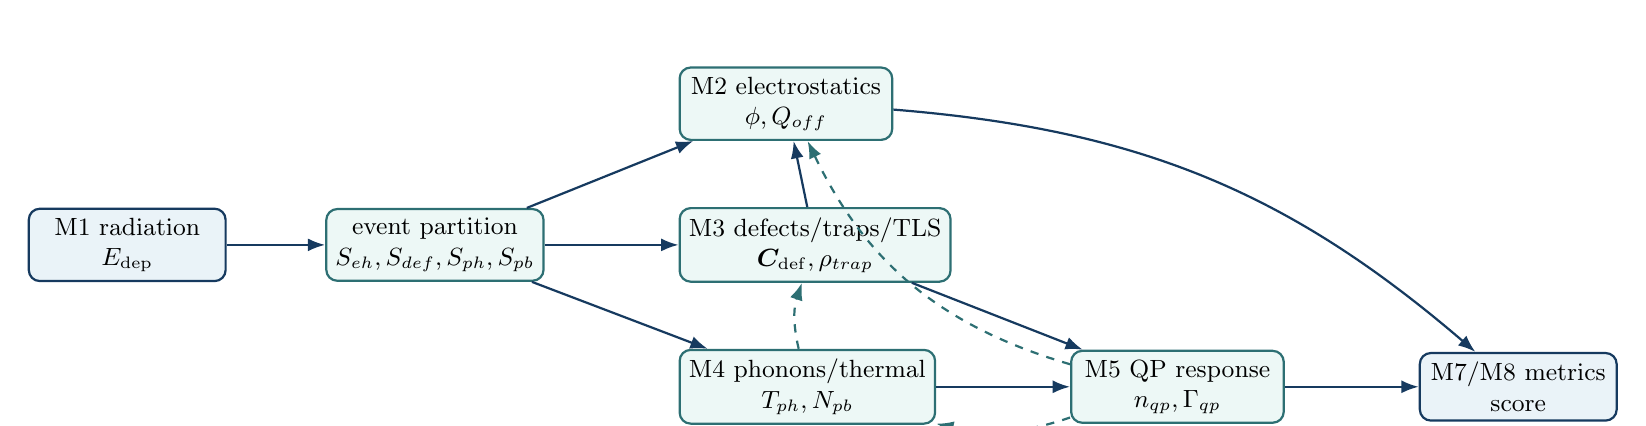
\begin{tikzpicture}[
node distance=1.1cm and 1.25cm,
box/.style={draw=TitleBlue,thick,rounded corners,align=center,fill=SoftBlue,minimum width=2.5cm,minimum height=0.78cm,font=\small},
smallbox/.style={draw=AccentTeal,thick,rounded corners,align=center,fill=SoftTeal,minimum width=2.7cm,minimum height=0.78cm,font=\small},
arrow/.style={-{Latex[length=2.2mm]},thick,draw=TitleBlue},
feedback/.style={-{Latex[length=2.2mm]},thick,dashed,draw=AccentTeal}
]

\node[box] (m1) {M1 radiation\\\(\Edep\)};
\node[smallbox,right=of m1] (part) {event partition\\\(S_{eh},S_{def},S_{ph},S_{pb}\)};
\node[smallbox,above right=0.85cm and 1.7cm of part] (m2) {M2 electrostatics\\\(\phi, Q_{off}\)};
\node[smallbox,right=1.7cm of part] (m3) {M3 defects/traps/TLS\\\(\Cvec,\rho_{trap}\)};
\node[smallbox,below right=0.85cm and 1.7cm of part] (m4) {M4 phonons/thermal\\\(T_{ph},N_{pb}\)};
\node[smallbox,right=1.7cm of m4] (m5) {M5 QP response\\\(n_{qp},\Gamma_{qp}\)};
\node[box,right=1.7cm of m5] (metrics) {M7/M8 metrics\\score};

\draw[arrow] (m1) -- (part);
\draw[arrow] (part) -- (m2);
\draw[arrow] (part) -- (m3);
\draw[arrow] (part) -- (m4);
\draw[arrow] (m3) -- (m2);
\draw[arrow] (m3) -- (m5);
\draw[arrow] (m4) -- (m5);
\draw[arrow] (m5) -- (metrics);
\draw[arrow] (m2) to[bend left=18] (metrics);
\draw[feedback] (m5) to[bend left=16] (m4);
\draw[feedback] (m4) to[bend left=16] (m3);
\draw[feedback] (m5) to[bend left=24] (m2);
\end{tikzpicture}%
}

\vspace{0.4em}
{\small Solid arrows: primary forward coupling. Dashed arrows: feedback through recombination phonons, temperature-dependent rates, and optional charge-imbalance/junction effects.}
\end{center}

The graph says that Module 6 must pass more than numerical arrays. It must pass physically classified source terms:
\begin{align}
\Edep &\rightarrow S_{eh},\quad S_{\mathrm{def}},\quad S_{\mathrm{ph}},\quad S_{\mathrm{pb}},\\
\Cvec &\rightarrow \rho_{\mathrm{trap}},\quad \DeltaSC(\Cvec),\quad \Dqp(\Cvec),\quad \Ic(\Cvec),\\
(\Tph,\Npb) &\rightarrow \Gqp,\quad \Gamma_{\mathrm{trap}},\quad D_{\mathrm{def}}(T),\\
(\nqp,\Qoff) &\rightarrow \Gammaqp,\quad \Gammaone,\quad \Gammaerr.
\end{align}

\section{Event partition: the new front end of Module 6}

A radiation event deposits energy. In a normal semiconductor model, one may map \(\Edep\) into electron-hole generation and defect production. In a superconducting-device model, the same deposited energy must be partitioned into several channels:
\begin{equation}
\Edep
=E_{eh}+E_{\mathrm{def}}+E_{\mathrm{ph,<pb}}+E_{\mathrm{ph,pb}}+E_{\mathrm{escape}}+E_{\mathrm{other}}.
\end{equation}
The pair-breaking phonon branch is especially important because phonons generated in the substrate can propagate far and create quasiparticles in superconducting electrodes.

Define partition fractions
\begin{equation}
\eta_{eh}+\eta_{\mathrm{def}}+\eta_{\mathrm{ph,<pb}}+\eta_{\mathrm{ph,pb}}+\eta_{\mathrm{escape}}+\eta_{\mathrm{other}}=1.
\end{equation}
Then the reduced source terms may be written
\begin{align}
S_{eh}(\x,t) &= \frac{\eta_{eh}\edot(\x,t)}{\varepsilon_{eh}},\\
S_{\mathrm{def}}(\x,t) &= \eta_{\mathrm{def}}\,Y_{\mathrm{def}}(\x)\,\edot(\x,t),\\
S_{\mathrm{ph}}(\x,t) &= \eta_{\mathrm{ph,<pb}}\edot(\x,t),\\
S_{\mathrm{pb}}(\x,t) &= \frac{\eta_{\mathrm{ph,pb}}\edot(\x,t)}{\langle \hbar\omega_{\mathrm{pb}}\rangle}.
\end{align}
Here \(\varepsilon_{eh}\) is the average energy required to create an electron-hole pair in the relevant substrate or dielectric, and \(Y_{\mathrm{def}}\) is a displacement or trap-production yield. These parameters are material- and radiation-dependent. They should be treated as calibration inputs until the project includes microscopic transport/downconversion models.

\begin{notebox}
\textbf{Do not overinterpret the partition fractions.} The \(\eta\)'s are reduced-model closure parameters. They are not constants of nature. They depend on particle type, energy, geometry, substrate, film stack, metallization, phonon escape, defects, and packaging.
\end{notebox}

\section{Coupled residual formulation}

A clean way to define Module 6 is through coupled residuals. Let
\begin{equation}
\state=\left(\state_2,\state_3,\state_4,\state_5\right)
\end{equation}
with
\begin{align}
\state_2 &= (\phiE,\Qoff,\Vvec),\\
\state_3 &= (\Cvec_{\mathrm{str}},\Nt,\ft,P_{\TLS},\DeltaSC,\Ic),\\
\state_4 &= (\Tph,\Npb),\\
\state_5 &= (\nqp,\Gammaqp,\Gammaone,\Gammaerr).
\end{align}
The coupled problem is
\begin{equation}
\boxed{
\mathcal{R}(\state;\Edep,\mathrm{geometry},\mathrm{BCs},\mathrm{parameters})=
\begin{bmatrix}
\Rtwo(\state_2;\state_3,\state_4,\state_5)\\
\Rthree(\state_3;\state_2,\state_4,\state_5,\Edep)\\
\Rfour(\state_4;\state_3,\state_5,\Edep)\\
\Rfive(\state_5;\state_2,\state_3,\state_4)
\end{bmatrix}=\bm{0}.}
\end{equation}
This is the most compact mathematical definition of superconducting Module 6.

\subsection{Module 2 residual inside Module 6}

The electrostatic residual in dielectric and substrate regions is
\begin{equation}
\Rtwo^{\Omega}(\phiE)=
-\nabla\cdot(\epsilon\nabla\phiE)
-\rho_{\mathrm{tot}}(\Cvec,\ft,\rho_{eh},\mustar),
\qquad \x\in\Osub\cup\Oox.
\end{equation}
The total charge density may be decomposed as
\begin{equation}
\rho_{\mathrm{tot}}
=\rho_{\mathrm{fixed}}+\rho_{\mathrm{trap}}(\Nt,\ft)+\rho_{eh}+\rho_{\mathrm{TLS}}+\rho_{\mathrm{imb}}.
\end{equation}
The charge-imbalance term \(\rho_{\mathrm{imb}}\) is optional. It is only meaningful if the model explicitly includes nonequilibrium quasiparticle charge imbalance. Most first-pass implementations should set it to zero.

For a superconducting island \(a\), an additional charge constraint is
\begin{equation}
R_{2,a}^{\mathrm{island}}
=Q_a-\sum_b C_{ab}V_b-Q_{a,\mathrm{off}}=0.
\end{equation}
The offset charge induced by a volume charge distribution can be computed with a weighting potential:
\begin{equation}
\boxed{
Q_{a,\mathrm{off}}(t)=\int_{\Osub\cup\Oox}\rhooff(\x,t)\,\wpot_a(\x)\,d\Omega .}
\end{equation}
The coupling point is clear: Module 3 supplies \(\rhooff\), Module 2 supplies \(\wpot_a\), and Module 5 consumes \(Q_{a,\mathrm{off}}\) through device-level charge sensitivity.

\subsection{Module 3 residual inside Module 6}

A material-resolved structural-defect residual has the form
\begin{equation}
R_{3,j}^{\mathrm{str}}
=\pdv{C_j}{t}
-\nabla\cdot(D_j(T,\Cvec)\nabla C_j)
-S_j(\Edep,T,\sigma,\mathrm{mat})
+R_j(\Cvec,T,\phiE),
\end{equation}
where \(S_j\) is a radiation-driven production term and \(R_j\) represents annealing, clustering, passivation, or conversion reactions.

Trap occupation is often better written as a local kinetic residual:
\begin{equation}
R_3^{\mathrm{trap}}
=\pdv{\ft}{t}
-c_{\mathrm{cap}}(\phiE,T,\rho_{eh})(1-\ft)
+e_{\mathrm{em}}(T,\phiE)\ft.
\end{equation}
The electrostatic charge density passed to Module 2 is
\begin{equation}
\rho_{\mathrm{trap}}(\x,t)=q_t\Nt(\x,t)\ft(\x,t),
\end{equation}
where \(q_t\) is the effective trap charge state.

Superconducting-film disorder maps enter through closures such as
\begin{align}
\DeltaSC(\x,t) &= \Delta_0\,F_{\Delta}(\Cvec_{\mathrm{film}},T),\\
\Tc(\x,t) &= T_{c0}\,F_c(\Cvec_{\mathrm{film}}),\\
\Dqp(\x,t) &= D_{\qp,0}\,F_D(\ell(\Cvec_{\mathrm{film}}),\DeltaSC),\\
\Ic(\x,t) &= I_{c0}\,F_I(\Cvec_{\mathrm{JJ}},\DeltaSC,T).
\end{align}
These are not solved by Module 3 alone; Module 6 owns the act of passing them into Modules 4 and 5.

\subsection{Module 4 residual inside Module 6}

A reduced phonon thermal residual can be written
\begin{equation}
R_4^{\mathrm{ph}}
=\Cph(T)\pdv{\Tph}{t}
-\nabla\cdot(\kappaph(T,\Cvec)\nabla\Tph)
-P_{\mathrm{dep}}
-P_{\mathrm{rec}}
+P_{\mathrm{pair}}
+P_{\mathrm{esc}}.
\end{equation}
The sign convention is model-dependent. One consistent convention is:
\begin{itemize}[leftmargin=2em]
\item \(P_{\mathrm{dep}}>0\): radiation energy added to the phonon bath;
\item \(P_{\mathrm{rec}}>0\): recombination energy emitted from QPs into phonons;
\item \(P_{\mathrm{pair}}>0\): high-energy phonon energy removed from the phonon branch to create QPs;
\item \(P_{\mathrm{esc}}>0\): energy lost to package, bath, traps, or downconversion structures.
\end{itemize}
A pair-breaking phonon population residual may be written as
\begin{equation}
R_4^{\mathrm{pb}}
=\pdv{\Npb}{t}
-\nabla\cdot(D_{\mathrm{pb}}\nabla\Npb)
-S_{\mathrm{pb}}
-\alpha_{\mathrm{rec}}\Rqp\nqp^2
+\Gammapb\Npb
+\frac{\Npb}{\tau_{\mathrm{esc}}}.
\end{equation}
Here \(\alpha_{\mathrm{rec}}\Rqp\nqp^2\) generates pair-breaking phonons through QP recombination, while \(\Gammapb\Npb\) removes high-energy phonons by breaking Cooper pairs.

\subsection{Module 5 residual inside Module 6}

A reduced QP residual in superconducting films is
\begin{equation}
R_5^{\mathrm{qp}}
=\pdv{\nqp}{t}
-\nabla\cdot(\Dqp(\Cvec,\DeltaSC,T)\nabla\nqp)
-\Gqp(\Npb,\Tph,\Edep)
+\Rqp\nqp^2
+\frac{\nqp}{\tautrap(\Cvec)}.
\end{equation}
The QP generation closure may be as simple as
\begin{equation}
\Gqp=2\Gammapb\Npb,
\end{equation}
because one broken Cooper pair creates two quasiparticles. More detailed models should include energy-dependent phonons and energy-dependent QP distributions.

Device metrics can then be reduced closures such as
\begin{align}
\Gammaqp^{(a)}(t) &= K_{\qp}^{(a)}\int_{\Omega_{\mathrm{sc},a}} W_a(\x)\nqp(\x,t)\,d\Omega,\\
\Gammaone^{(a)}(t) &= \Gamma_{1,0}^{(a)}+\Gamma_{1,\qp}^{(a)}(\nqp)+\Gamma_{1,\TLS}^{(a)}(P_{\TLS}),\\
\Gammaerr^{(a)}(t) &= F_{\mathrm{err}}\left(\Gammaone^{(a)},\Gammaqp^{(a)},\Qoff^{(a)},\delta\DeltaSC^{(a)}\right).
\end{align}
The weighting factor \(W_a\) maps a spatial QP density to the sensitivity of device \(a\). It may be an electrode mask, junction-local sensitivity map, resonator-current weighting map, or a learned surrogate.

\section{Time-scale separation}

A central reason Module 6 must be redesigned is that the coupled variables evolve on very different time scales.

\begin{center}
\rowcolors{2}{SoftGray}{white}
\begin{tabularx}{\textwidth}{p{0.24\textwidth}p{0.22\textwidth}X}
\toprule
\textbf{Variable/process} & \textbf{Typical role} & \textbf{Coupling consequence}\\
\midrule
Electrostatic potential \(\phiE\) & Quasi-static field & Usually solved instantaneously relative to defect or QP evolution.\\
Substrate charge collection/trapping & Event transient to slow trapping & Needs event update plus relaxation/trap kinetics.\\
Pair-breaking phonons & Fast nonlocal excitation branch & Couples radiation deposition to QP generation far from impact site.\\
Quasiparticle density \(\nqp\) & Fast to intermediate poisoning state & Evolves dynamically and feeds device error metrics.\\
Trap/TLS occupations & Slow stochastic or activated dynamics & Feeds offset-charge noise and dielectric loss.\\
Structural disorder \(\Cvec\) & Very slow at cryogenic temperature & Often updated event-by-event, not by smooth thermal diffusion.\\
Thermal bath \(\Tph\) & Depends on geometry and bath coupling & May be quasi-static for average heating or dynamic for pulses.\\
\bottomrule
\end{tabularx}
\end{center}

This suggests a multi-rate algorithm. Let \(t_m\) denote slow material-update times and \(\tau\) denote fast post-event time. For each radiation event or dose increment:
\begin{enumerate}[leftmargin=2em]
\item Update slow structural/trap state only if the event creates persistent damage.
\item Solve or update quasi-static electrostatics for \(\phiE\) and \(\Qoff\).
\item Evolve fast phonon and QP branches over \(\tau\).
\item Integrate device metrics over the relevant measurement window.
\item Update cumulative degradation or scoring variables.
\end{enumerate}

\section{Fixed-point iteration strategy}

A practical Module 6 implementation can use a staggered fixed-point iteration. At global step \(m\), define the old coupled state
\begin{equation}
\state^m=(\phiE^m,\Qoff^m,\Cvec^m,\rho_{\mathrm{trap}}^m,\Tph^m,\Npb^m,\nqp^m,\Gamma^m).
\end{equation}
For a dose step or event update, perform inner iterations \(k=0,1,2,\ldots\):
\begin{align}
\textbf{M3:}\quad
(\Cvec,\rho_{\mathrm{trap}},P_{\TLS})^{k+1}
&=\Mthree(\Edep,\Tph^k,\phiE^k,\nqp^k),\\
\textbf{M2:}\quad
(\phiE,\Qoff,\Vvec)^{k+1}
&=\Mtwo(\rho_{\mathrm{trap}}^{k+1},\Cvec^{k+1},\mathrm{BCs}),\\
\textbf{M4:}\quad
(\Tph,\Npb)^{k+1}
&=\Mfour(\Edep,\Cvec^{k+1},\nqp^k),\\
\textbf{M5:}\quad
(\nqp,\Gammaqp,\Gammaone,\Gammaerr)^{k+1}
&=\Mfive(\Npb^{k+1},\phiE^{k+1},\Qoff^{k+1},\Cvec^{k+1},\Tph^{k+1}).
\end{align}
A relaxed update improves stability:
\begin{equation}
\state^{k+1}\leftarrow (1-\omega)\state^k+\omega\state^{k+1}_{\mathrm{raw}},
\qquad 0<\omega\le 1.
\end{equation}
The convergence metric should not be only \(\|\phiE^{k+1}-\phiE^k\|\). It should include the quantities that matter for superconducting performance:
\begin{equation}
\epsilon_{\mathrm{couple}}=
\max\left(
\frac{\|\phiE^{k+1}-\phiE^k\|}{\|\phiE^k\|+\epsilon},
\frac{|\Qoff^{k+1}-\Qoff^k|}{|\Qoff^k|+\epsilon},
\frac{\|\nqp^{k+1}-\nqp^k\|}{\|\nqp^k\|+\epsilon},
\frac{|\Gammaerr^{k+1}-\Gammaerr^k|}{|\Gammaerr^k|+\epsilon}
\right).
\end{equation}

\section{Monolithic residual strategy}

For strongly coupled cases, Module 6 can instead define one nonlinear residual and solve it monolithically:
\begin{equation}
\mathcal{R}(\state)=\bm{0}.
\end{equation}
Newton's method would require the Jacobian
\begin{equation}
\mathcal{J}=\pdv{\mathcal{R}}{\state}
=\begin{bmatrix}
\pdv{\Rtwo}{\state_2} & \pdv{\Rtwo}{\state_3} & \pdv{\Rtwo}{\state_4} & \pdv{\Rtwo}{\state_5}\\
\pdv{\Rthree}{\state_2} & \pdv{\Rthree}{\state_3} & \pdv{\Rthree}{\state_4} & \pdv{\Rthree}{\state_5}\\
\pdv{\Rfour}{\state_2} & \pdv{\Rfour}{\state_3} & \pdv{\Rfour}{\state_4} & \pdv{\Rfour}{\state_5}\\
\pdv{\Rfive}{\state_2} & \pdv{\Rfive}{\state_3} & \pdv{\Rfive}{\state_4} & \pdv{\Rfive}{\state_5}
\end{bmatrix}.
\end{equation}
This is elegant but probably too heavy for the next MATLAB implementation stage. The block structure is still valuable because it identifies which feedbacks are physically important.

\begin{center}
\rowcolors{2}{SoftGray}{white}
\begin{tabularx}{\textwidth}{p{0.18\textwidth}p{0.38\textwidth}X}
\toprule
\textbf{Jacobian block} & \textbf{Physical meaning} & \textbf{Keep in first reduced model?}\\
\midrule
\(\partial \Rtwo/\partial \state_3\) & Trap/TLS charge modifies electrostatics & Yes.\\
\(\partial \Rthree/\partial \state_4\) & Temperature controls defect/trap kinetics & Yes, if thermal feedback is active.\\
\(\partial \Rfour/\partial \state_5\) & QP recombination emits phonons & Yes for QP pulse modeling.\\
\(\partial \Rfive/\partial \state_4\) & Pair-breaking phonons generate QPs & Essential.\\
\(\partial \Rfive/\partial \state_3\) & Disorder changes QP diffusion/trapping/JJ parameters & Yes in degradation studies.\\
\(\partial \Rtwo/\partial \state_5\) & QP charge imbalance modifies electrostatics & Usually no for first model.\\
\bottomrule
\end{tabularx}
\end{center}

\section{Energy conservation across Modules 4 and 5}

The most important coupling consistency check is energy conservation between the phonon branch and the QP branch. If \(\nqp\) denotes QP number density near the gap edge, the QP energy density is approximately
\begin{equation}
U_{\qp}\approx \DeltaSC\nqp.
\end{equation}
A more detailed model would integrate the energy-dependent distribution, but this gap-edge approximation is appropriate for a reduced Module 6 note.

The QP energy equation implied by the QP number equation is
\begin{equation}
\pdv{U_{\qp}}{t}
\approx \DeltaSC\left[\nabla\cdot(\Dqp\nabla\nqp)+\Gqp-\Rqp\nqp^2-\frac{\nqp}{\tautrap}\right]
+\nqp\pdv{\DeltaSC}{t}.
\end{equation}
If pair-breaking phonons create QPs, the phonon energy loss must match the QP energy gain:
\begin{equation}
P_{\mathrm{pair}}\approx \DeltaSC G_{\qp}.
\end{equation}
If two QPs recombine into a Cooper pair and emit a phonon of energy approximately \(2\DeltaSC\), then the phonon energy gain is
\begin{equation}
P_{\mathrm{rec}}\approx \DeltaSC R_{\qp}\nqp^2,
\end{equation}
assuming \(R_{\qp}\nqp^2\) is written as a loss rate of QP number. The exact factor depends on whether the recombination coefficient is defined for QP pairs or QP number loss. Module 6 should enforce one convention globally.

\begin{physicsbox}
\textbf{Module 6 convention recommendation.} Define \(\Rqp\nqp^2\) as the number loss rate of QPs per volume per time. Then the QP equation contains \(-\Rqp\nqp^2\), and the energy transferred from QPs to phonons is \(\DeltaSC\Rqp\nqp^2\). This avoids repeated factors of two in the code.
\end{physicsbox}

\section{Charge conservation and offset-charge consistency}

The superconducting extension introduces two different meanings of charge:
\begin{enumerate}[leftmargin=2em]
\item physical charge density in dielectric/substrate regions, which sources Poisson's equation;
\item induced island offset charge, which affects the superconducting circuit Hamiltonian.
\end{enumerate}
These must not be confused. A trapped charge distribution \(\rhooff(\x,t)\) produces electrostatic fields through Module 2 and also induces island charge through a weighting potential:
\begin{equation}
Q_{a,\mathrm{off}}=\int \rhooff\wpot_a\,d\Omega.
\end{equation}
The same trapped charge should not be counted twice. A safe Module 6 rule is:
\begin{itemize}[leftmargin=2em]
\item use \(\rhooff\) in Poisson's equation to compute \(\phiE\);
\item use the weighting-potential integral to compute \(\Qoff\);
\item pass only \(\Qoff\) to the circuit/device-response closure, not \(\rhooff\) again unless the response model explicitly requires local electric field sensitivity.
\end{itemize}

The dimensionless island charge is
\begin{equation}
\ngate(t)=\frac{C_gV_g+\Qoff(t)}{2e}.
\end{equation}
For charge-sensitive devices, radiation-induced \(\delta\ngate\) can produce frequency shifts, parity changes, or changes in relaxation depending on operating point and device design.

\section{Material-parameter coupling closures}

Module 6 must own the maps from Module 3 structural state to Module 4/5 coefficients. Typical closures include
\begin{align}
\kappaph(\x,T,t)&=\kappa_{0}(T)\,F_{\kappa}(\Cvec_{\mathrm{str}},\mathrm{interfaces}),\\
\Dqp(\x,t)&=D_{\qp,0}\,F_D(\ell(\Cvec_{\mathrm{film}}),\DeltaSC,T),\\
\tautrap^{-1}(\x,t)&=\tau_{\mathrm{trap},0}^{-1}+K_{\mathrm{trap}}\,N_{\mathrm{trap}}(\x,t),\\
\DeltaSC(\x,t)&=\Delta_0\,F_{\Delta}(\Cvec_{\mathrm{film}},T),\\
\Ic(t)&=I_{c0}\,F_I(\Cvec_{\mathrm{JJ}},\DeltaSC,T),\\
\Gamma_{\TLS}(t)&=F_{\TLS}(P_{\TLS},\Evec,\omega_q,T).
\end{align}
The functions \(F\) can start as empirical scalings or user-defined closures. The key architecture point is that these maps should not be buried inside independent modules. If buried, the same defect field may be interpreted inconsistently by electrostatics, thermal transport, and QP response.

\section{Boundary and interface coupling}

The superconducting coupling layer also changes boundary conditions.

\subsection{Electrostatic interfaces}

At a dielectric-superconductor interface, the potential is continuous and the normal displacement jumps by surface charge:
\begin{align}
\phiE_{\mathrm{dielectric}}&=V_{\mathrm{sc}},\\
\nnormal\cdot(\epsilon\nabla\phiE)_{\mathrm{dielectric}}&=-\sigma_s.
\end{align}
For an ideal grounded superconducting electrode, \(V_{\mathrm{sc}}=0\). For a floating island, \(V_{\mathrm{sc}}\) is determined by a charge constraint.

\subsection{Thermal interfaces}

At a substrate-film or film-bath boundary, a Kapitza-type condition can be written
\begin{equation}
-\nnormal\cdot\kappaph\nabla T_{\mathrm{sub}}
=G_K(T_{\mathrm{sub}}-T_{\mathrm{film}}).
\end{equation}
At very low temperature and for short pulses, a spectral boundary condition may be more appropriate than this local-temperature approximation. In a reduced MATLAB model, \(G_K\) can be used as the first closure.

\subsection{QP interfaces}

At a superconducting film boundary, QPs may reflect, trap, escape, or tunnel. A reduced Robin condition is
\begin{equation}
-\nnormal\cdot \Dqp\nabla\nqp=s_{\mathrm{trap}}\nqp-s_{\mathrm{emit}}.
\end{equation}
At a Josephson junction, QP tunneling can be modeled as a boundary sink/source:
\begin{equation}
-\nnormal\cdot \Dqp\nabla\nqp = \Gamma_{\mathrm{tun}}(\nqp,\delta,\DeltaSC,T).
\end{equation}
This boundary flux couples Module 5 to device poisoning metrics.

\section{Recommended superconducting Module 6 algorithm}

For the next implementation stage, a robust algorithm is more important than a maximal physics model. A recommended reduced algorithm is:

\begin{enumerate}[leftmargin=2em]
\item \textbf{Load geometry and material regions.} Identify \(\Osub\), \(\Oox\), \(\Osc\), and \(\Ojj\). Store material labels per mesh element.
\item \textbf{Load Module 1 deposition.} Convert energy-deposition bins to a source object.
\item \textbf{Partition event energy.} Compute \(S_{eh}\), \(S_{\mathrm{def}}\), \(S_{\mathrm{ph}}\), and \(S_{\mathrm{pb}}\).
\item \textbf{Update persistent defects/traps.} Run Module 3 update for \(\Cvec\), \(\Nt\), \(\ft\), and \(\rho_{\mathrm{trap}}\).
\item \textbf{Solve hybrid electrostatics.} Run Module 2 to obtain \(\phiE\), \(\wpot\), and \(\Qoff\).
\item \textbf{Evolve phonon branch.} Run Module 4 to obtain \(\Tph\) and \(\Npb\).
\item \textbf{Evolve QP branch.} Run Module 5 to obtain \(\nqp\), \(\Gammaqp\), and \(\Gammaone\).
\item \textbf{Evaluate device metrics.} Compute qubit/resonator degradation, correlated-error score, and reduced scoring metrics.
\item \textbf{Check convergence or advance event.} Repeat the coupled update if strong feedback is enabled.
\end{enumerate}

\subsection{Pseudocode}

\begin{verbatim}
state = initialize_superconducting_state(mesh, materials, params)
for event = 1:numEvents
    src = partition_deposited_energy(Edep(event), params.partition)

    for k = 1:maxCouplingIterations
        old = state

        state.defects = module3_sc_update(src.defect, state.Tph, state.phi, params)
        state.rhoTrap = traps_to_charge(state.defects, state.traps)

        state.electrostatics = module2_sc_solve(mesh, state.rhoTrap, params)
        state.Qoff = compute_offset_charge(state.electrostatics.weighting, state.rhoTrap)

        state.thermal = module4_sc_update(src.phonon, state.nqp, state.defects, params)
        state.Npb = state.thermal.Npb
        state.Tph = state.thermal.Tph

        state.qp = module5_sc_update(state.Npb, state.Qoff, state.defects, state.Tph, params)
        state.metrics = device_metrics_sc(state.qp, state.Qoff, state.defects, params)

        if coupled_change(state, old) < params.couplingTol
            break
        end
        state = relax_state(old, state, params.omegaRelax)
    end
end
\end{verbatim}

\section{PINN and causal-PINN implications}

The superconducting Module 6 extension changes what a PINN or CPINN surrogate should learn. A single neural network surrogate for \(\phiE(x,y)\) is no longer enough if the goal is coupled superconducting response. Candidate surrogate maps include
\begin{align}
\mathcal{G}_2 &: (\rho_{\mathrm{trap}},\mathrm{BCs},\mathrm{geometry})\mapsto (\phiE,\Qoff),\\
\mathcal{G}_4 &: (S_{\mathrm{ph}},S_{\mathrm{pb}},\mathrm{geometry})\mapsto (\Tph,\Npb),\\
\mathcal{G}_5 &: (\Npb,\Dqp,\tautrap,\mathrm{geometry})\mapsto (\nqp,\Gammaqp),\\
\mathcal{G}_6 &: (\Edep,\Cvec,\rho_{\mathrm{trap}},\mathrm{geometry})\mapsto (\Qoff,\nqp,\Gammaerr).
\end{align}

For CPINN, the natural causal coordinate is not physical time in the Poisson problem alone. In Module 6, however, several valid orderings exist:
\begin{itemize}[leftmargin=2em]
\item post-event time \(\tau\) for phonon/QP evolution;
\item dose step or event count for cumulative damage;
\item coupling iteration index for self-consistent convergence;
\item energy-downconversion stage from high-energy phonons to thermal phonons;
\item geometry-continuation parameter for mitigation structures.
\end{itemize}
A causal loss for Module 6 can group residuals by event time windows:
\begin{equation}
\mathcal{L}_{\mathrm{CPINN},6}
=\sum_{m=1}^{N_t} w_m
\left(
\lambda_2\mathcal{L}_{2,m}
+\lambda_3\mathcal{L}_{3,m}
+\lambda_4\mathcal{L}_{4,m}
+\lambda_5\mathcal{L}_{5,m}
+\lambda_c\mathcal{L}_{\mathrm{couple},m}
\right),
\end{equation}
with
\begin{equation}
 w_m=\exp\left[-\epsilon_c\sum_{r=1}^{m-1}\mathcal{L}_r\right].
\end{equation}
Here \(\mathcal{L}_{\mathrm{couple},m}\) penalizes violation of interface, energy-conservation, offset-charge, and QP-generation consistency conditions.

\section{Verification tests for superconducting Module 6}

The future MATLAB implementation should not be trusted until the following tests pass.

\subsection{Test 1: zero-radiation equilibrium}

Set \(\Edep=0\), no trap charge, and no pair-breaking phonon source. The solver should return
\begin{equation}
\Qoff=0,
\qquad
\nqp\approx n_{\qp,\mathrm{eq}}(T),
\qquad
\Gammaerr\approx \Gamma_{\mathrm{background}}.
\end{equation}
No artificial QP source should appear from the coupling loop.

\subsection{Test 2: pure trapped-charge event}

Inject a static trapped charge distribution but no pair-breaking phonons. Then
\begin{equation}
\Qoff\ne 0,
\qquad
\nqp\approx n_{\qp,\mathrm{background}}.
\end{equation}
This test checks that Module 6 does not incorrectly convert electrostatic trapped charge into QPs.

\subsection{Test 3: pure phonon-only event}

Inject \(S_{\mathrm{pb}}\ne0\) but no ionizing trapped charge. Then
\begin{equation}
\Qoff\approx0,
\qquad
\nqp(t)>0.
\end{equation}
This test is important because recent superconducting-qubit experiments show phonon-mediated QP poisoning can occur even when offset-charge shifts are not the dominant event signature.

\subsection{Test 4: energy-conservation check}

For a closed reduced system with no escape and fixed \(\DeltaSC\), the combined phonon plus QP energy should satisfy
\begin{equation}
\dv{}{t}\int_{\Omega}\left(U_{\mathrm{ph}}+\DeltaSC\nqp\right)d\Omega
=\int_{\Omega}\edot\,d\Omega.
\end{equation}
Numerical deviations should decrease with time-step refinement.

\subsection{Test 5: spatial footprint check}

A localized substrate impact should produce a nonlocal QP poisoning footprint if pair-breaking phonons propagate efficiently. Adding a downconversion or trapping layer should reduce and localize the footprint.

\subsection{Test 6: coupling convergence check}

For a steady dose-rate problem, the fixed-point iteration should converge monotonically or at least stably under relaxation. If convergence depends sensitively on update order, the code should report the coupling residuals by module.

\section{Suggested MATLAB data structures}

A superconducting Module 6 implementation should store coupling variables explicitly. A possible MATLAB structure is:

\begin{verbatim}
state_sc.phi              % electrostatic potential field
state_sc.E                % electric field
state_sc.Qoff             % island offset charges
state_sc.weighting        % weighting potentials for islands

state_sc.defects.C        % structural defect species
state_sc.defects.trapRho  % trap charge density
state_sc.defects.tls      % TLS/disorder descriptors
state_sc.defects.Delta    % superconducting gap map
state_sc.defects.Ic       % junction critical-current map

state_sc.thermal.Tph      % phonon temperature/effective energy
state_sc.thermal.Npb      % pair-breaking phonon population
state_sc.thermal.power    % power partition and escape terms

state_sc.qp.nqp           % quasiparticle density
state_sc.qp.Dqp           % QP diffusivity map
state_sc.qp.Gqp           % QP generation map
state_sc.qp.tauTrap       % QP trapping/removal time

state_sc.metrics.Gamma_qp % QP poisoning/parity rate
state_sc.metrics.Gamma_1  % relaxation rate
state_sc.metrics.Qscore   % reduced superconducting degradation score
\end{verbatim}

The coupling configuration should also be explicit:

\begin{verbatim}
params_sc.coupling.enableElectrostaticFeedback = true
params_sc.coupling.enableThermalFeedback       = true
params_sc.coupling.enableQPRecombinationPhonons = true
params_sc.coupling.enableChargeImbalance       = false
params_sc.coupling.maxIterations               = 20
params_sc.coupling.tolerance                   = 1e-4
params_sc.coupling.relaxation                  = 0.5
\end{verbatim}

\section{Connection to Modules 7 and 8}

Although this note is about Module 6, the coupling layer should be designed with Module 7 and Module 8 in mind. The superconducting device-response outputs should include both field-level and scalar metrics:
\begin{align}
Y_{\mathrm{SC}}(t)=
\left[
\Qoff(t),\nqp(\x,t),\Gammaqp(t),\Gammaone(t),\delta f_q(t),\delta Q_i(t),\Gammaerr(t)
\right].
\end{align}
A superconducting reduced score may have the form
\begin{equation}
S_{\mathrm{SC}}=
w_Q\frac{\|\Qoff\|}{Q_{\mathrm{ref}}}
+w_{\qp}\frac{\int \nqp W\,d\Omega}{N_{\mathrm{ref}}}
+w_1\frac{\Gammaone-\Gamma_{1,0}}{\Gamma_{1,0}+\epsilon}
+w_c\,P_{\mathrm{corr}}.
\end{equation}
Here \(P_{\mathrm{corr}}\) is a correlated-error or multi-device poisoning metric. This metric is not part of ordinary semiconductor degradation, but it is central for superconducting qubit arrays.

\section{What should change in the project architecture}

The practical implication is that Module 6 should eventually become two layers:

\begin{enumerate}[leftmargin=2em]
\item \textbf{Physics coupling layer.} Responsible for residuals, source partition, state passing, fixed-point/monolithic iteration, conservation checks, and material closures.
\item \textbf{Application wrapper.} Selects normal semiconductor mode or superconducting-device mode.
\end{enumerate}

The normal and superconducting modes should not be forced into the same variable names. A clean project structure would be
\begin{verbatim}
module6_coupling_normal.m
module6_coupling_superconducting.m
module6_partition_radiation_event_sc.m
module6_update_state_sc.m
module6_check_conservation_sc.m
module6_compute_metrics_sc.m
\end{verbatim}
This avoids contaminating the normal silicon degradation model with superconducting variables that do not belong there.

\section{Summary}

The superconducting-region extension changes Module 6 from a conventional multiphysics coupling loop into a multi-branch event-response architecture. The normal model couples electrostatics, defect evolution, heat, and carrier transport. The superconducting model must couple:
\begin{itemize}[leftmargin=2em]
\item hybrid electrostatics and superconducting island offset charge;
\item structural defects, traps, TLSs, and disorder maps;
\item substrate phonons, pair-breaking phonons, and cryogenic thermal boundaries;
\item quasiparticle diffusion, recombination, trapping, and tunneling;
\item Josephson-device degradation metrics and correlated-error scores.
\end{itemize}

The central design rule is separation of physical branches. Structural damage is not the same thing as quasiparticles. Trapped charge is not the same thing as offset charge, although it induces offset charge. Heat is not one scalar temperature when pair-breaking phonons and QPs are dynamically important. The job of superconducting Module 6 is to keep these variables separate while enforcing charge, energy, interface, and device-response consistency.

\begin{physicsbox}
\textbf{Final modeling conclusion.} The first useful superconducting Module 6 implementation should not attempt a full microscopic superconductor simulation. It should implement a reduced but physically separated coupling loop:
\begin{equation}
\Edep\rightarrow
(S_{\mathrm{trap}},S_{\mathrm{pb}},S_{\mathrm{def}})
\rightarrow
(\Qoff,\Npb,\nqp)
\rightarrow
(\Gammaqp,\Gammaone,\Gammaerr).
\end{equation}
That architecture is simple enough to code in MATLAB and rich enough to capture the radiation-specific superconducting failure pathways.
\end{physicsbox}

\section*{References and source anchors}
\addcontentsline{toc}{section}{References and source anchors}

This project note is a derived modeling document, not a literature review. The following sources are useful anchors for the physical mechanisms emphasized here:
\begin{enumerate}[leftmargin=2em]
\item E. Yelton et al., ``Modeling phonon-mediated quasiparticle poisoning in superconducting qubit arrays,'' arXiv:2402.15471, 2024.
\item C. P. Larson et al., ``Quasiparticle poisoning of superconducting qubits with active gamma irradiation,'' arXiv:2503.07354, 2025.
\item V. Iaia et al., ``Phonon downconversion to suppress correlated errors in superconducting qubits,'' arXiv:2203.06586, 2022.
\item X. Li et al., ``Cosmic-ray-induced correlated errors in superconducting qubit arrays,'' Nature Communications, 2025.
\item A. Rothwarf and B. N. Taylor, ``Measurement of recombination lifetimes in superconductors,'' Physical Review Letters, 1967. This is the classic source for the coupled quasiparticle/phonon recombination-pair-breaking picture.
\end{enumerate}

\end{document}
